\chapter{Metodologia}
\label{cap:metodologia}

Nossos experimentos seguem rigidamente o processo descrito em \citep{Elahi:2014:ALS:2542182.2542195}, uma vez que este é o trabalho mais completo sobre o tema em questão. Há, contudo, uma importante diferença que deve ser ressaltada. Os autores em \citep{Elahi:2014:ALS:2542182.2542195} abordam a questão da \textit{Elicitação de Preferências para fins de Arranque Frio}, com isso, não podem assumir que os usuários avaliarão todos os itens solicitados. É possível que eles desconheçam algum dos itens (ou até mesmo todos) solicitados pela estratégia de AA, tanto que o percentual de preferências adquiridas é uma das métricas utilizadas para se medir o desempenho das estratégias.

Em nosso trabalho, pelo contrário, já que estamos abordando o problema de \textit{Elicitação de Preferências para fins de Incentivo}, podemos assumir que os usuários avaliarão todos os itens solicitados pela estratégia. Esta suposição se sustenta pelo fato de que os itens solicitados serão sempre itens que já foram adquiridos pelos usuários, além, claro, da existência de um incentivo individual para quando os usuários contribuem com suas preferências.

\section{Nomenclatura} 

A fim de mantermos a relação com \citep{Elahi:2014:ALS:2542182.2542195} ainda mais estreita, optamos por utilizar boa parte da nomenclatura que este usa ao descrever seus experimentos. Assim, o leitor que desejar ler os dois trabalhos não terá problema algum para perceber a correspondência entre ambos e poderá compará-los com extrema facilidade.

Como de costume, os problemas referentes a SR fazem uso de uma matriz esparsa como sendo a estrutura que representa as preferências dos usuários em relação aos itens. Nossa entrada é, portanto, uma matriz $R$, de $n$ usuários por $m$ itens ($n\times m$), onde cada posição preenchida $r_{ij}$ representa a nota dada pelo usuário $i$ ao item $j$. Conforme esperado, o numero de posições preenchidas da matriz $R$ é uma pequena fração do numero total de posições $n\times m$, o que a classifica como esparsa.

$R$ é dividida em duas matriz disjuntas $T$ e $Tr$, com as mesmas dimensões, a primeira contendo 20\% das avaliações de $R$ e a segunda com os remanescentes 80\%. A matriz $T$ será usada para fins de teste, enquanto que $Tr$ será novamente divida em $K$ e $X$, com 5\% e 95\% de $Tr$, respectivamente. Todas essas divisões são realizadas de maneira aleatória.

Para utilizarmos uma técnica de recomendação, ou modelo, é necessário que haja uma base de preferências ainda que limitada. Desta forma, $K$ é inicializada com 5\% da base original, representando as preferências conhecidas pelo sistema em um momento inicial. $X$, por sua vez, contem as preferências que serão adquiridas pelo sistema, i.e., os itens que os usuários compraram, porém não avaliaram explicitamente. As preferências contidas em $X$ serão elicitadas através de uma estratégia $S$ e, uma vez elicitadas, serão colocadas em $K$, incrementando o conhecimento do sistema.

Uma estratégia $S(i, N, K, C_i)$ é uma função que, dado um determinado usuário $i$, atribui uma pontuação para os itens dentro do conjunto $C_i$. Tal conjunto representa os itens que o usuário $i$ adquiriu, porém não avaliou. Logo, são itens passíveis de serem solicitados pela estratégia, i.e., $C_i \subset X_i$, onde $X_i$ representa a linha da matriz $X$ correspondente ao usuário $i$. A pontuação dada por $S$, normalmente, é fruto de alguma heurística calculada com base nas preferências conhecidas até então pelo sistema (matriz $K$). O retorno de $S$ é uma lista $L$ contendo os $N$ itens com maior pontuação. Caso o numero de itens em $C_i$ seja menor que $N$, retorna-se todos os itens de $C_i$.

\section{Experimentos}

Primeiramente, é necessário definir o número de itens ($N$) que serão elicitados a cada iteração e o número total de iterações ($it$) a serem executadas. Em nossos experimentos, utilizamos $N=10$ e $it=50$. O numero de usuários ($n$) e itens de ($m$) varia conforme a base de dados que será utilizada.

Com a finalidade de garantirmos certa segurança estatística em nossos resultados, realizamos a \textit{validação cruzada} com 5 partições. Ou seja, dividimos a matriz $R$ em 5 partições disjuntas, todas com o mesmo número de preferências, chamadas de $R_y$, e repetimos o procedimento principal 5 vezes. A cada rodada, utilizou-se uma das partições, contento 20\% de $R$, como sendo o conjunto teste $T$ e as demais como sendo o conjunto de treinamento $Tr$.

O procedimento principal, por sua vez, inicia-se quando alocamos aleatoriamente 5\% das preferências de $Tr$ para $K$ e o restante para $X$. Durante $it$ iterações, empregamos uma estratégia $S$ para buscar os melhores $N$ itens, que, quando avaliados pelo usuário $i$, trarão o maior ganho de acurácia para o modelo. A preferência de $i$ por tais itens é então elicitada, o que, na prática, significa que as avaliações de $i$ referentes aos itens em $L$ são removidas de $X$ e acrescentadas em $K$. Feito isto para todos os usuários, treinamos o modelo $\theta$ com a matriz $K$, agora com novas preferências, e o utilizamos para prever as preferências contidas em $T$.

O Erro Médio Absoluto das previsões, em inglês, \textit{Mean Absolute Error} (MAE), descrito na seção \ref{sec:modelo-avaliacao}, é calculado e armazenado com sendo o erro referente à iteração e à rodada. Ao fim de todas as rodadas, calculamos a média e o desvio padrão dos erros a cada iteração para que, desta maneira, resultados muito discrepantes sejam amenizados.

Um esquema completo de nosso experimento pode ser visto no algoritmo \ref{alg:exp-completo}. Nele, a função $RAND$ é responsável por alocar 5\% das preferências de $Tr$ para $K$; a função $\Gamma$ é responsável calcular o MAE do modelo $\theta$, treinado com a matrix $K$, no conjunto de teste $T$; as funções $MEAN$ e $STD$ são responsáveis por calcular a média e o desvio padrão, respectivamente; e por $ERROR[:, z]$, denotamos toda a coluna $z$ da matriz $ERROR$. 

Como estamos interessados em comparar o desempenho de diversas estratégias de AA, o procedimento descrito no algoritmo \ref{alg:exp-completo} foi aplicado para um total de 17 estratégias, incluindo a \textit{Estratégia Livre de Viés}. Uma descrição de cada uma delas pode ser encontrada na seção \ref{sec:estrategias} e os resultados de nossos experimentos serão apresentados e discutidos no capítulo \ref{cap:resultados}.

\begin{algorithm}
\caption{Procedimento para se avaliar uma estratégia $S$} 
\begin{algorithmic}[1]
\State{$N \gets 10$} \Comment{Número de itens retornados}
\State{$it \gets 50$} \Comment{Número de iterações}
\For{$y$}{$1$}{$5$} \Comment{Rodadas da validação cruzada}
  \State{$T \gets R_y$}
  \State{$Tr \gets R \setminus R_y$}
  \State{$K \gets RAND(Tr, 5\%)$}
  \State{$X \gets Tr \setminus K$}
  \For{$t$}{$1$}{$it$}
    \For{$i$}{$1$}{$n$}
        \State{$C_i \gets X_i > 0$} \Comment{Itens cujas preferências podem ser elicitadas}
        \State{$L \gets S(i, N, K, C_i)$}
        \State{$K \gets K + L$}
        \State{$X \gets X \setminus L$}
    \EndFor
    \State{$ERROR[y, t] \gets \Gamma(\theta(K), T)$} \Comment{Avaliação do desempenho de $S$}
  \EndFor
\EndFor
\For{$z$}{$1$}{$it$} \Comment{Estatísticas da validação cruzada}
    \State{$media[z] = MEAN(ERROR[:, z])$}
    \State{$desvio[z] = STD(ERROR[:, z])$}
\EndFor
\end{algorithmic}
\label{alg:exp-completo}
\end{algorithm}

\section{Modelo e Métrica de Avaliação}
\label{sec:modelo-avaliacao}

Conforme visto no capítulo \ref{cap:fundamentacao}, diversos algoritmos foram propostos para a tarefa de prever as preferência dos usuários. Em particular, mencionamos que os modelos baseados na decomposição SVD se sobressaíram aos demais, não apenas por causa dos bons resultados, mas, sobretudo, devido a capacidade do SVD gerar um espaço vetorial customizável onde usuários e itens podem ser mapeados. Ou seja, tais modelos além de fornecerem as previsões, possibilitam que os projetistas do SR compreendam melhor os usuários e itens conforme suas disposições dentro do espaço gerado. 

Para calcular as previsões, optamos pelo modelo baseado em SVD conhecido como \textit{Regularized SVD}, descrito na seção \ref{sec:regularized-svd}. Conforme aconselhado por \citep{paterek_2007}, utilizamos $\rho=0,001$, $\lambda=0,02$, $\varepsilon=0,1$ e $k=96$. Na prática, poderíamos ter utilizado qualquer modelo capaz de fazer previsões paras as tuplas (usuário, item) presentes em $T$, uma vez que não estamos interessados em obter o menor erro possível, e sim avaliar como o decaimento do erro se comporta dependendo da estratégia escolhida.

Em \citep{Elahi:2014:ALS:2542182.2542195}, os autores utilizam o modelo descrito em \citep{KorenBell_2011}. Ambos são baseados na decomposição SVD, a única diferença é que o modelo de \citep{KorenBell_2011} faz uso da média global ($\mu$), do viés do usuário ($bias_i$) e do viés do item ($bias_j$) para o cálculo de previsão. Neste sentido, ele é mais parecido com o \textit{Improved Regularized SVD}, descrito na seção \ref{sec:improved-regularized-svd}, do que com o \textit{Regularized SVD}. Apesar de apresentar resultados levemente superiores, nossa opção pelo \textit{Regularized SVD} se justifica pela simplicidade de implementação, já que não é necessário atualizar os parâmetros $bias_i$ e $bias_j$.

Todavia, para afirmar que um modelo apresenta desempenho bom ou ruim, é preciso que haja uma métrica capaz de avaliá-lo. Nos problemas relacionados a SR, duas métricas se popularizaram dentro da literatura, são elas o Erro Médio Absoluto, em inglês, \textit{Mean Absolute Error} (MAE); e a Raiz de Erro Médio Quadrático, em inglês, \textit{Root Mean Square Error} (RMSE) \citep{ricci_recommender_2011}. Vale ressaltar que ambas as técnicas visam avaliar o sistema como um todo, tratando todas as previsões como possuindo igual importância. Há casos onde deseja-se avaliar a capacidade do modelo fazer previsões para um grupo específico de usuários ou itens, ou então, deseja-se avaliar a capacidade do modelo prever determinados valores de preferência. Nesses casos não é recomendado fazer uso do MAE nem do RMSE, no entanto, como em nossos experimentos estamos interessados no desempenho global do sistema, tanto MAE quanto RMSE são métricas apropriadas.

Por outro lado, utilizar ambas as técnicas seria redundante, visto que, em essência, elas traduzem a mesma informação, que é a diferença média entre a previsão dada pelo modelo e a verdadeira preferência contida no conjunto de teste. Portanto, optamos por medir nossos resultados apenas com o MAE a fim de podermos realizar comparações mais diretas com \citep{Elahi:2014:ALS:2542182.2542195}, que também acatou pela mesma métrica.

Quanto ao cálculo propriamente dito, seja $\hat{r}_{ij}$ a previsão dada pelo modelo para a preferência do usuário $i$ pelo item $j$, ambos pertencentes ao conjunto de teste $T$; e seja $r_{ij}$ a verdadeira preferência deste usuário pelo item. Assim, o valor de MAE é dado segundo a equação \ref{eq:mae}, enquanto que o valor de RSME é dado segundo a equação \ref{eq:rmse}. 

\begin{equation}
MAE = \sum_{(i,j) \in T} |r_{ij} - \hat{r}_{ij}|
\label{eq:mae}
\end{equation}

\begin{equation}
RMSE = \sqrt{\sum_{(i,j) \in T} (r_{ij} - \hat{r}_{ij})^2}
\label{eq:rmse}
\end{equation}

\section{Base de Dados}

A primeira base escolhida foi a \textit{MovieLens 100k}, ou simplesmente \textit{MovieLens}, disponibilizada pelo grupo \textit{GroupLens} \citep{Herlocker:1999:AFP:312624.312682}. Esta base contem 100 mil preferências, oriundas de 943 usuários e 1682 itens, que, neste caso, representam filmes. Logo, ela contem apenas 6,3\% de todas as possíveis preferências, sendo que 6.110 possuem valor igual a 1; 11.370 igual a 2; 27.145 igual a 3; 34.174 igual a 4; e 21.201 igual a 5.

A segunda base escolhida foi a do desafio \textit{Netflix} \citep{Bennett07thenetflix}. Completa, esta base possui possui mais de 100 milhões de preferências, o que torna inviável a execução de nossos experimentos. Realizamos portanto um ``corte'', coletando as 100 mil primeiras preferências fornecidas. Este corte é oriundo de 1.499 usuários e 2.382 itens, também filmes, sendo que o numero de preferências corresponde a apenas 2,8\% do total possível. Dessas preferências, 8.149 possuem valor igual 1; 14.253 igual a 2; 34.503 igual 3; 27.076 igual a 4; e 16.019 igual 5.

Há várias bases de recomendação, abordando inúmeros tipos de itens, porém, as bases apresentadas nesta seção são muito bem conhecidas dentro da literatura, havendo diversos trabalhos que fazem uso das mesmas. Além disso, ambas são utilizadas em \citep{Elahi:2014:ALS:2542182.2542195}, inclusive, o corte da base \textit{Netflix} foi proposto por este trabalho.

\section{Estratégias comparadas}
\label{sec:estrategias}

Definir quais estratégias serão utilizadas e avaliadas em nossos experimentos é, por si só, uma tarefa árdua, visto não há um consenso claro dentro da literatura sobre quais estratégias servem como referência para o problema abordado. Aliás, o problema em si foi pouco explorado dentro da literatura de SR. 

Mesmo quando tratamos do problema análogo, a \textit{Elicitação de Preferências para fins de Arranque Frio}, ainda não existem referências bem consolidadas, com exceção da estratégia aleatória. Todavia, há estratégias que se popularizaram pelo fato de terem sido usadas em trabalhos importantes da área. Decidimos portanto escolher 16 estratégias para comparação com a \textit{Estratégia Livre de Viés}, algumas sendo as mais ``populares'' da literatura e outras sendo combinações dessas.

\subsection{\textit{random}}
A estratégia \textit{random} é a estratégia mais básica possível, ou seja, \textit{random} pode ser interpretada como sendo a ausência de estratégia. Assim, para uma estratégia $S$ ser considerada minimamente eficaz, ela deve ter desempenho, no mínimo, melhor que \textit{random}. Em nosso caso, utilizar a estratégia \textit{random} consiste em selecionar, de forma aleatória, $N$ itens dentre os que estão presentes no conjunto $C_i$.

\subsection{\textit{popularity}}
Esta estratégia se propõe a ordenar os itens de acordo com o seu valor de popularidade. Para calcular a popularidade de um item, verifica-se quantos usuários já avaliaram este item. Em termos formais, a função que determina o valor de popularidade do item $j$, $pop(j)$, é dada conforme a equação \ref{eq:popularity}. Calculamos então o valor de $pop$ para todos os itens em $C_i$ e solicitamos que o usuário avalie os $N$ itens com maior popularidade. 

\begin{equation}
pop(j) = \sum_{i \in K, r_{ij} > 0} 1
\label{eq:popularity}
\end{equation}

\subsection{\textit{entropy}}
A estratégia \textit{entropy} visa ordenar os itens com base no seu valor de entropia. Proposta pela primeira vez em \citep{Rashid:2002:GKY:502716.502737}, a estratégia busca associar a entropia de um determinado item ao consenso médio que os usuários possuem sobre este item. Entretanto, neste mesmo trabalho, os autores afirmam que esta relação só pode ser traçada caso o item possua um valor significativo de popularidade. A função $ent(j)$ retorna o valor de entropia para o item $j$, onde $r$ representa o valor das possíveis avaliações em $K$, e $p_j(r)$ a probabilidade do item $j$ receber a nota $r$.

\begin{equation}
ent(j) = -\sum_{r \in K, r > 0} p_j(r) \log p_j(r)
\label{entropy}
\end{equation}

\subsection{\textit{entropy0}}
As deficiências de se utilizar apenas a entropia pura são extensamente abordadas em \citep{Rashid:2008:LPN:1540276.1540302}. Em linhas gerais, não se pode tirar conclusões sobre a entropia de itens com baixa popularidade. Para contornar tal problema, \citep{Rashid:2008:LPN:1540276.1540302} propõe incorporar a ``impopularidade'' do item no cálculo da entropia, considerando as avaliações com valor 0. Contudo, como o número de avaliações 0 é muito superior as outras, atribui-se um peso maior para as avaliações positivas. Esta estratégia ficou conhecida como \textit{entropy0} e a função que exprime sua fórmula é dada através da equação \ref{eq:entropy0}, onde $w_r$ representa o peso da nota $r$. Em nossos experimentos utilizamos $w_0=0,5$ e $w_1=w_2=w_3=w_4=w_5=1$.

\begin{equation}
ent0(j) = \frac{- \sum_{r \in K} w_r p_j(r) \log p_j(r)}{\sum_{r \in K} w_r}
\label{eq:entropy0}
\end{equation}

\subsection{\textit{log(pop)*ent}}
Uma maneira alternativa de se amenizar as deficiências da entropia pura é combinar seu valor com a popularidade do item. Assim, itens com alta entropia, mas que possuem baixa popularidade, seriam penalizados e itens de alta entropia, com também alta popularidade, seriam destacados. Esta é solução proposta por \citep{Rashid:2002:GKY:502716.502737}, porém os autores verificaram que o valor bruto da popularidade iria prevalecer sobre o valor da entropia, logo, ao invés disso, propuseram o logaritmo da popularidade. A equação \ref{eq:log(pop)*ent} mostra o cálculo de \textit{log(pop)*ent}.

\begin{equation}
logpopent(j) = \log pop(j) \times ent(j)
\label{eq:log(pop)*ent}
\end{equation}

\subsection{\textit{log(pop)*ent0}}
Apesar de nenhum trabalho apresentar esta combinação, optamos por combinar a popularidade com \textit{entropy0} de maneira análoga à combinação realizada em \textit{log(pop)*ent}. Desta forma, criou-se a estratégia \textit{log(pop)*ent0}, cuja fórmula é dada pela equação \ref{eq:log(pop)*ent0}.

\begin{equation}
logpopent0(j) = \log pop(j) \times ent0(j)
\label{eq:log(pop)*ent0}
\end{equation}

\subsection{\textit{helf}}
Outra maneira de se combinar o logaritmo da popularidade e a entropia pura é apresentado em \citep{Rashid:2008:LPN:1540276.1540302}. Nele, ao invés da simples multiplicação, optou-se por calcular a média harmônica das funções $\log pop$ e $ent$, uma medida muito conhecida na área de RI \citep{Baeza-Yates:1999:MIR:553876}. A grosso modo, tanto \textit{helf} quanto \textit{log(pop)*ent} são implementações diferentes de uma mesma ideia, que é tentar amenizar as desvantagens individuais de cada estratégia através da combinação de ambas. A equação \ref{eq:helf} apresenta a fórmula para o cálculo de \textit{helf}, onde $n$ é o número total de usuários e $r_{max}$ é o maior valor de preferência que um usuário pode dar. 

\begin{equation}
helf(j) = \frac{2 \times (\log pop(j)/\log n) \times (ent(j)/\log r_{max})}{(\log pop(j)/\log n) + (ent(j)/\log r_{max})}
\label{eq:helf}
\end{equation}

\subsection{\textit{helf0}}
Semelhantemente ao caso de \textit{log(pop)*ent0}, criamos uma estratégia que utiliza a média harmônica para combinar os valores $\log pop$ e $ent0$, a qual chamamos de \textit{helf0}. O seu cálculo se dá conforme a equação \ref{eq:helf0}.

\begin{equation}
helf0(j) = \frac{2 \times (\log pop(j)/\log n) \times (ent0(j)/\log r_{max})}{(\log pop(j)/\log n) + (ent0(j)/\log r_{max})}
\label{eq:helf0}
\end{equation}

\subsection{\textit{igcn}}
A estratégia \textit{igcn}, cujo nome é a sigla para \textit{Information Gain through Clustered Neighbors}, foi proposta em \citep{Rashid:2008:LPN:1540276.1540302} e se baseia no conceito do Ganho de Informação (GI). Este conceito procura mensurar a ``quantidade'' de informação que uma determinada variável agrega à resolução de um problema, tendo se tornado famoso por causa das \textit{Árvores de Decisão} \citep{Rokach:2008:DMD:1796114}. Na prática, o \textit{igcn} procura criar uma Árvore de Decisão que classifica os usuários em \textit{clusters}, de acordo com a nota que cada um deu a cada item.

%\abbrev{GI}{Ganho de Informação}

Primeiramente, aplica-se a decomposição SVD na matriz $K$ e, com isso, obtém-se um mapeamento dos usuários em um espaço vetorial de $\omega$ dimensões. A partir da disposição dos usuários nesse espaço, utilizamos um algoritmo de clusterização hierárquica para agrupar os usuários em $\varphi$ \textit{clusters}. Assim calculamos os itens que, quando avaliados, melhor distribuem os usuários em \textit{clusters}, ou seja, que trazem o maior decréscimo na entropia referente a distribuição dos usuários em \textit{clusters}. Tais itens são os que possuem maior GI.

Todavia, calcular o GI dos itens não uma tarefa trivial, tendo em vista que deve-se levar em consideração as avaliações de valor zero. Como essas superabundam em nossas bases, é preciso contrabalançar os efeitos de tais avaliações através de um peso artificial. A equação \ref{eq:igcn} apresenta como se dá o cálculo do \textit{igcn}, onde $|U|$ é a quantidade total de usuários; $|U_{j}^{r}|$ é a quantidade de usuários que avaliaram o item $j$ com nota $r$; $w_r$ é o peso referente a nota $r$; $H(U)$ é a entropia da distribuição de todos os usuários em \textit{clusters}; e $H(U_{j}^{r})$ é a entropia da distribuição dos usuários que avaliaram o item $j$ com nota $r$ em \textit{clusters}. 

Em nossos experimento, utilizamos $\omega=100$ e $\varphi=300$. Para facilitar o cálculo de $H(U)$ e $H(U_{j}^{r})$, consideramos apenas a distribuição em \textit{clusters} dos 150 usuários mais próximos do usuário $i$ \citep{Rashid:2008:LPN:1540276.1540302}. 

\begin{equation}
igcn(j) = H(U) - \sum_{r \in K} \frac{w_r \frac{|U_{j}^{r}|}{|U|}}{E(j)} H(U_{j}^{r})
\label{eq:igcn}
\end{equation}

\begin{equation}
E(j) = \sum_{r \in K} w_r \frac{|U_{j}^{r}|}{|U|}
\end{equation}

\subsection{\textit{variance}}
Esta estratégia busca ordenar os itens pela variância das avaliações recebidas. Em essência, ela está intimamente ligada a \textit{entropy}, uma vez que ambas procuram mensurar o consenso dos usuários sobre os itens através de uma medida de dispersão. Inclusive, a variância pura padece do mesmo problema que a entropia pura, i.e., quando o item possui poucas avaliações, tirar conclusões a respeito do valor de sua variância pode ser enganoso e, por esta razão, poucos trabalhos a utilizam. Apesar de \citep{Elahi:2014:ALS:2542182.2542195} afirmar que utilizou \textit{variance} em seus experimentos, este menciona que seus resultados não se destacaram e, por isto, não foram apresentados. Calculamos a variância de um item $j$ através da equação \ref{eq:variance}, onde $n$ é o numero de avaliações que o item $j$ recebeu e $\overline{r_{j}}$ é a média das mesmas.

\begin{equation}
var(j) = \frac{1}{(n-1)} \times \sum_{i \in K, r_{ij} > 0} (r_{ij} - \overline{r_{j}})^2
\label{eq:variance}
\end{equation}

\subsection{\textit{sqrt(pop)*var}}
Com o intuito de amenizar as desvantagens da variância pura, \citep{Golbandi:2010:BRS:1871437.1871734} propôs a combinar a variância com a popularidade, analogamente ao que foi proposto em \textit{log(pop)*ent}. Entretanto, ao invés de utilizar a escala logarítmica para os valores de popularidade, os autores optaram pelo uso da raiz quadrada desses valores. A equação \ref{eq:sqrt(pop)*var} apresenta a fórmula para o cálculo de \textit{sqrt(pop)*var}. 

\begin{equation}
sqrtpopvar(j) = \sqrt{pop(j)} \times var(j)
\label{eq:sqrt(pop)*var}
\end{equation}

\subsection{\textit{log(pop)*var}}
Apesar de não ter sido encontrado nenhum trabalho fazendo uso desta estratégia, julgamos cabível testar também o logaritmo da popularidade para se amenizar os efeitos da variância, conforme foi empreendido em \textit{log(pop)*ent}. A fórmula para se calcular esta estratégia, nomeada de \textit{log(pop)*var}, pode ser descrita segundo a equação \ref{eq:log(pop)*var}.

\begin{equation}
logpopvar(j) = \log pop(j) \times var(j)
\label{eq:log(pop)*var}
\end{equation}

\subsection{\textit{bin pred}}
A estratégia \textit{bin pred} (abreviação para \textit{Binary Prediction}) proposta em \citep{Elahi:2014:ALS:2542182.2542195}, procura prever quais itens o usuário irá consumir e, a partir de então, assume que será melhor para o sistema adquirir as avaliações a respeito desses itens. A previsão $\hat{b}_{ij}$ indica se o usuário $i$ irá consumir ou não o item $j$ e é calculada a partir da matriz binária $B$. Esta matriz, por sua vez, é gerada a partir da matriz $K$, de tal forma que as avaliações positivas de $K$ possuem valor 1 na matriz $B$ e as avaliações com valor zero são mantidas. O modelo descrito na seção \ref{sec:modelo-avaliacao} é treinado com a matriz $B$ e nos retorna previsões $\hat{b}_{ij}$ para todos os itens. Por fim, a estratégia solicita os $N$ itens em $C_i$ com maior previsão.

\subsection{\textit{high pred}}
Na mesma linha de \textit{bin pred}, \textit{high pred} (abreviação para \textit{Highest Predicted}) realiza o treinamento do modelo com a matriz $K$ e calcula as previsões $\hat{r}_{ij}$ para as notas faltantes. Os $N$ itens em $C_i$ com as maiores previsões são solicitados ao usuário $i$. Esta estratégia, também proposta em \citep{Elahi:2014:ALS:2542182.2542195}, assume que é melhor para o SR adquirir as avaliações altas do que as baixas.

\subsection{\textit{low pred}}
Ao contrário de \textit{high pred}, \textit{low pred} (abreviação para \textit{Lowest Predicted}) assume que é melhor para o SR solicitar as avaliações baixas em detrimento das altas \citep{Elahi:2014:ALS:2542182.2542195}. O funcionamento de \textit{low pred} se assemelha muito ao de \textit{high pred}, o modelo é treinado com a matriz $K$ e as previsões para as notas faltantes $\hat{r}_{ij}$ são calculadas. Feito isso, calcula-se uma nova previsão dada por $\hat{\alpha}_{ij} = r_{max}-\hat{r}_{ij}$, onde $r_{max}$ é o maior valor de preferência que um usuário pode dar. Solicita-se então os $N$ itens de $C_i$ com maior previsão $\hat{\alpha}_{ij}$.

\subsection{\textit{high-low pred}}
Por último, temos a estratégia \textit{high-low pred}, proposta em \citep{Elahi:2014:ALS:2542182.2542195}, que nada mais é do que uma tentativa de se combinar \textit{high pred} e \textit{low pred}. Analogamente a essas, utiliza-se o modelo, treinado com a matriz $K$, a fim de se calcular as previsões $\hat{r}_{ij}$ para as notas faltantes. A partir de então, calcula-se uma nova previsão dada por $\hat{\beta}_{ij} = |\frac{r_{max}+r_{min}}{2}-\hat{r}_{ij}|$, que indica o quão distante a previsão está do valor médio ($r_{max}$ e $r_{min}$ são os valores máximo e mínimo de preferência, respectivamente). Escolhe-se os $N$ itens pertencentes a $C_i$ com maior valor de $\hat{\beta}_{ij}$.

\section{Parametrização}
\label{sec:escolha-parametros}

Conforme comentado na seção \ref{sec:parametrizacao} a escolha dos parâmetros da \textit{Estratégia Livre de Viés} (o numero de dimensões $k$ e a largura da janela $\sigma$) foi realizada de maneira empírica, analisando o comportamento da estratégia para diversos valores diferentes. Definido um valor de $k$, avaliamos qual o valor de $\sigma$ que resulta no melhor desempenho da estratégia, lembrando que o eixo vertical representa o MAE enquanto que o eixo horizontal representa o numero de iterações ($it=15$). 

Apesar das comparações entre as estratégias terem sido realizadas em duas bases diferentes, os testes para escolha de parâmetros foram realizados apenas na base \textit{MovieLens}. Além disso, com a finalidade de simplificar a notação, nos referimos aos valores de $\sigma$ como sendo escalares. No entanto, $\sigma$ é uma matriz quadrada $k \times k$ cujas posições da diagonal principal possuem o valor mencionado. Por exemplo, se $k = 2$, quando mencionamos $\sigma=0,5$ isto significa que $\sigma = \bigl(\begin{smallmatrix} 0,5&0\\ 0&0,5 \end{smallmatrix} \bigr)$.

A figura \ref{fig:2dimensions} apresenta o desempenho da \textit{Estratégia Livre de Viés} com diversos valores de $\sigma$ para $k=2$. Como é possível observar, há uma pequena vantagem quando utilizamos $\sigma=0,00005$ nas primeiras 8 iterações. Da mesma forma, na figura \ref{fig:3dimensions}, onde $k=3$, vemos que $\sigma=0,00005$ ainda resulta no melhor desempenho, porém a vantagem em relação as outras é bem mais sutil.  

\begin{figure}[ht]
\centering
\includegraphics{2dimensions.eps}
\caption{Comparação de diferentes $\sigma$'s utilizando $k=2$}
\label{fig:2dimensions}
\end{figure}

\begin{figure}[ht]
\centering
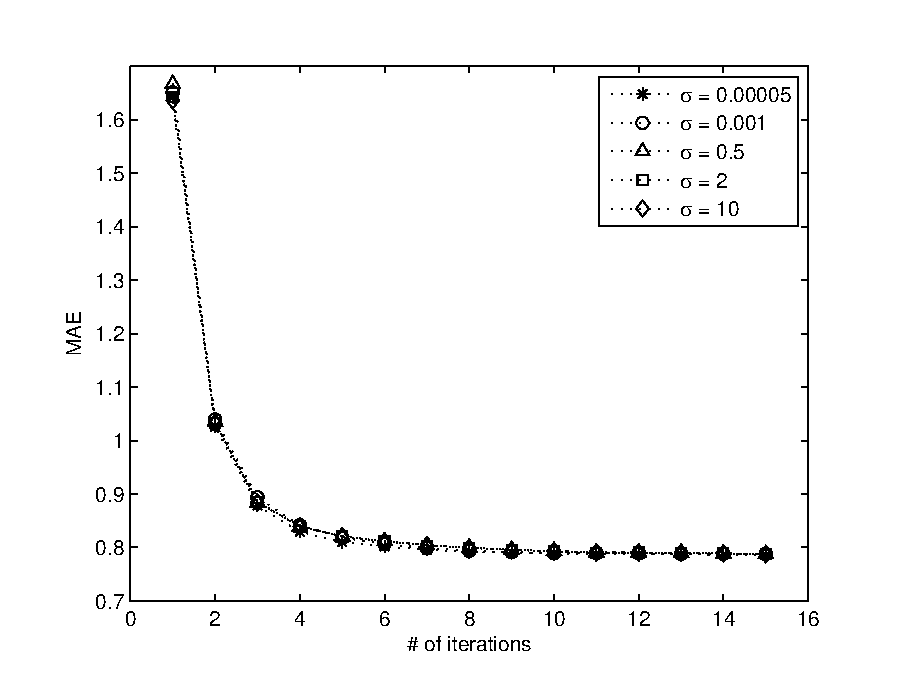
\includegraphics{3dimensions.eps}
\caption{Comparação de diferentes $\sigma$'s utilizando $k=3$}
\label{fig:3dimensions}
\end{figure}

Na figura \ref{fig:5dimensions}, onde $k=5$, novamente temos desempenhos muito próximos, entretanto notamos que, nas primeiras 4 iterações, $\sigma=10$ é melhor, enquanto que, a partir da 8ª iteração, $\sigma=0,00005$ é melhor. Já na figura \ref{fig:10dimensions}, onde $k=10$, $\sigma=10$ é claramente melhor. Por fim, quando tomamos $k=50$, na figura \ref{fig:50dimensions}, temos novamente o melhor resultado com $\sigma=0,00005$.

\begin{figure}[ht]
\centering
\includegraphics{5dimensions.eps}
\caption{Comparação de diferentes $\sigma$'s utilizando $k=5$}
\label{fig:5dimensions}
\end{figure}

\begin{figure}[ht]
\centering
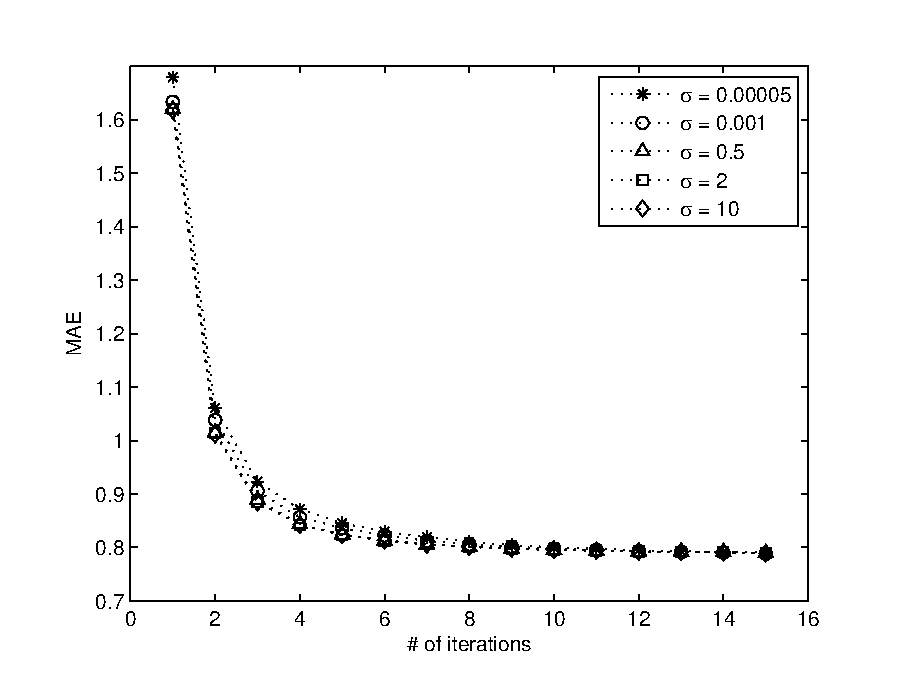
\includegraphics{10dimensions.eps}
\caption{Comparação de diferentes $\sigma$'s utilizando $k=10$}
\label{fig:10dimensions}
\end{figure}

\begin{figure}[ht]
\centering
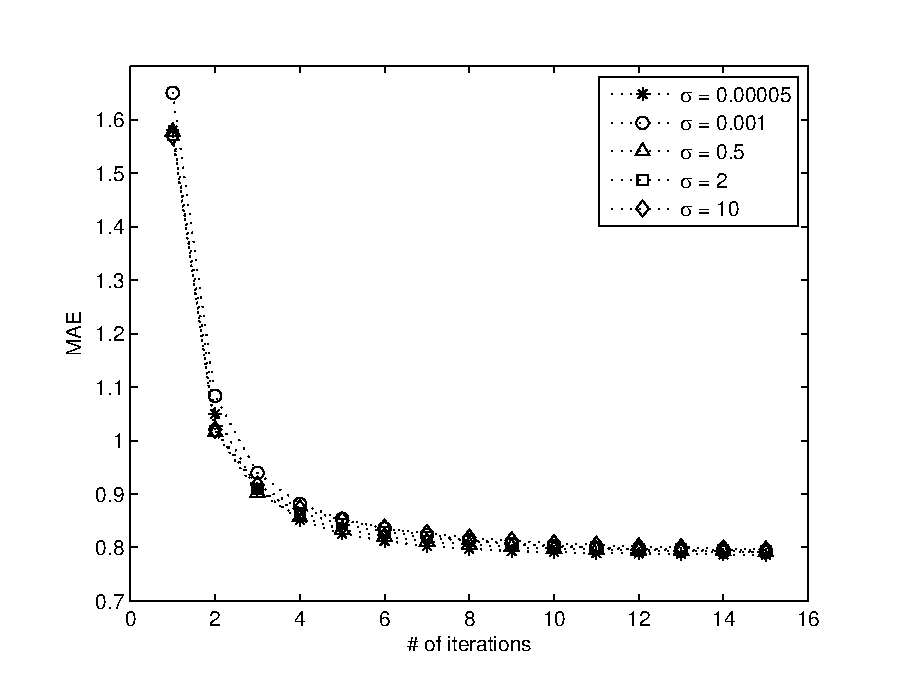
\includegraphics{50dimensions.eps}
\caption{Comparação de diferentes $\sigma$'s utilizando $k=50$}
\label{fig:50dimensions}
\end{figure}

Dado um valor para $k$, podemos concluir que as variações de desempenho percebidas, ao se mudar o parâmetro $\sigma$, são mínimas. Contudo, a fim de visualizarmos as variações de desempenho resultantes das mudanças em $k$, apresentamos na figura \ref{fig:final} o desempenho da \textit{Estratégia Livre de Viés}, para cada valor de $k$ testado, com seu respectivo melhor valor de $\sigma$. Como é possível observar, o melhor resultado ocorre com $k=2$ e $\sigma=0,00005$ e foram esses os parâmetros escolhidos para a \textit{Estratégia Livre de Viés} que será comparada com as demais no capitulo \ref{cap:resultados}.

\begin{figure}[ht]
\centering
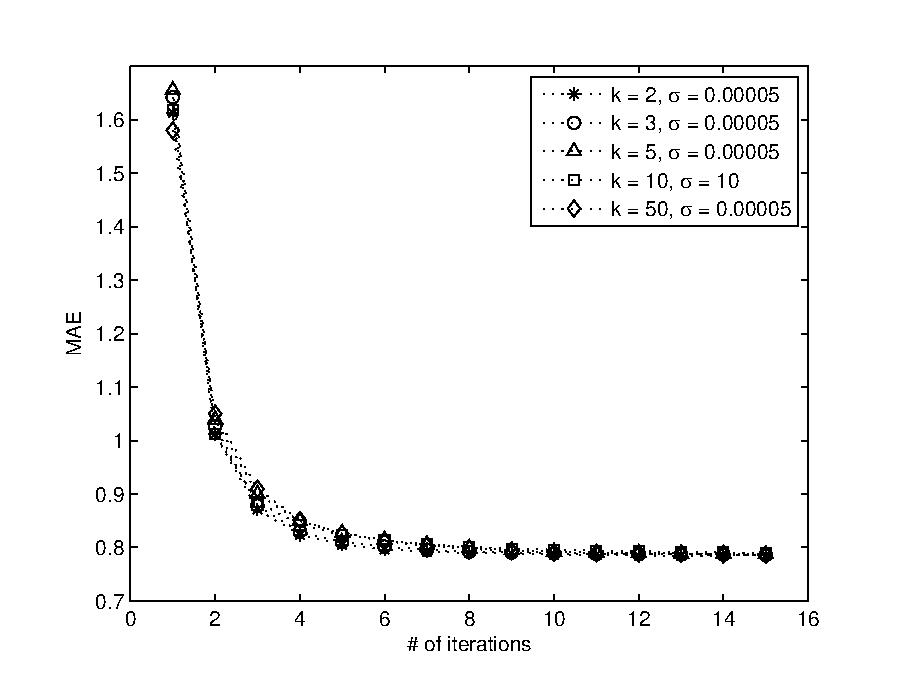
\includegraphics{final.eps}
\caption{Comparação de diferentes $k$'s com seus melhores $\sigma$'s}
\label{fig:final}
\end{figure}












